% !TEX root = Apostila GP.tex

\chapter{Gerenciamento de Integração}

\begin{figure}[!h]
\centering
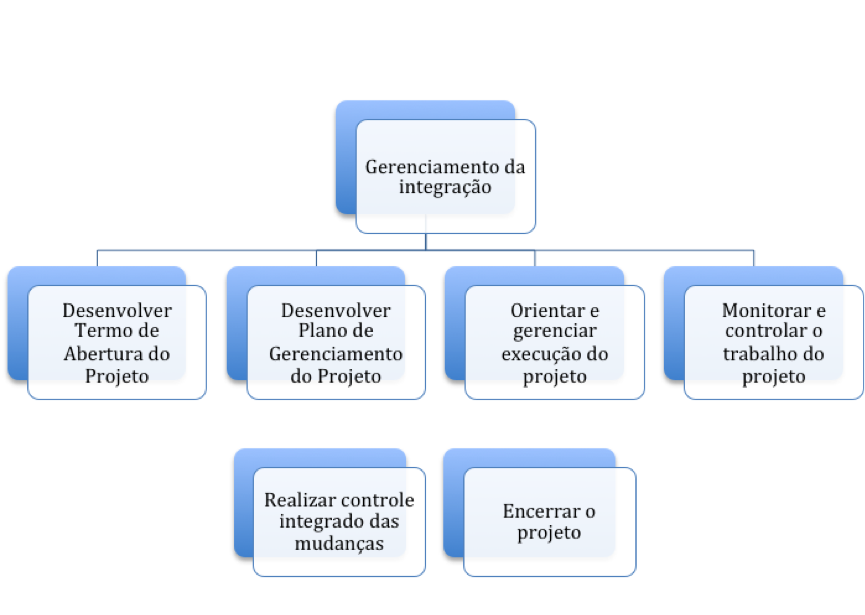
\includegraphics[scale=0.75]{Figuras/gerenciamento_integracao.png}
\caption{Processos do Gerenciamento da Integração}
\label{fig:proc:ger:integr}
\end{figure}

\section{\planproj}

O \planproj é um documento usado no auxílio da gerência do projeto no seu dia a dia. Ele é formalizado e aprovado pelos \stake e deve conter informações realistas sobre o projeto.

Ele é composto por:

\begin{itemize}

\item Plano do planejamento

\item Planos de gerenciamento de todas as áreas que serão controladas

\item Linha de base do escopo, cronograma e orçamento

\item Outros documentos e processos importantes para o gerenciamento do projeto

\end{itemize}

\subsection{Plano do planejamento}

É considerado como o pré-planejamento. Consiste em atribuir datas, responsáveis e tarefas com o objetivo de planejar o projeto e gerar os documentos e informações necessárias para a \kick. A Figura \ref{fig:plano:planejamento} mostra um exemplo de plano contendo algumas das tarefas mais importantes.

\begin{figure}[!h]
\centering
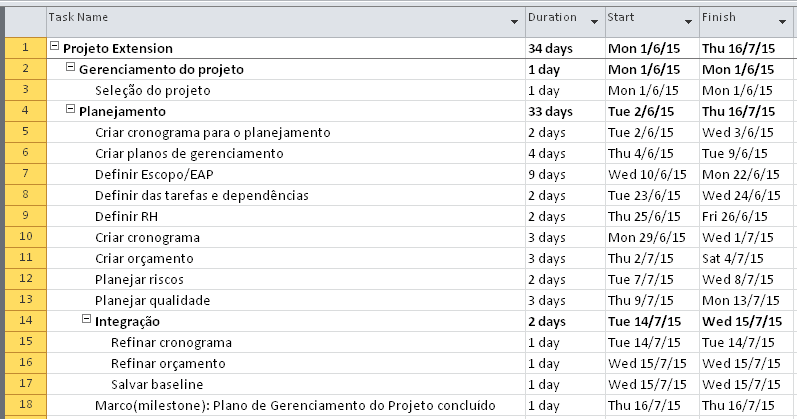
\includegraphics[scale=0.5]{Figuras/plano_planejamento.png}
\caption{Exemplo de Plano do Planejamento}
\label{fig:plano:planejamento}
\end{figure}

\subsection{\Kick}

É o evento que formaliza o início do projeto e que tem como um dos objetivos principais deixar claro os papéis e responsabilidades de todos no projeto. Por isso a participação de todos os \stake é de suma importância. Trata-se de uma ótima oportunidade de colocar frente a frente a equipe, clientes e outros \stake.

\subsection{Integracão dos planos}

Um projeto é como um organismo vivo no qual uma deficiência em uma área pode influenciar uma ou mais outras áreas. Quanto mais tarde essa deficiência for detectada e corrigida, piores serão as consequências.

Por este motivo, os planos de gerenciamento das diversas áreas do projeto não podem ser considerados totalmente independentes e devem ser construídos e mantidos de forma integrada.

Os planos de gerenciamento do projeto seguem as áreas de conhecimento que serão estudadas:

\begin{itemize}

\item \planesc
\item \plancron
\item \plancusto
\item \planqual
\item \planpess
\item \plancom
\item \planrisco
\item \planaq

\end{itemize}

Organizações que possuem escritórios de projeto (PMO) podem definir planos de gerenciamentos padronizados para que não se perca tempo com processos que se repetem em cada novo projeto. Neste caso, cabe ao \gp seguir os processos e planos definidos e o Plano do Planejamento vai incluir somente o cronograma das etapas.

\subsection{Processo Desenvolver o \planproj}

\begin{figure}[!h]
\centering
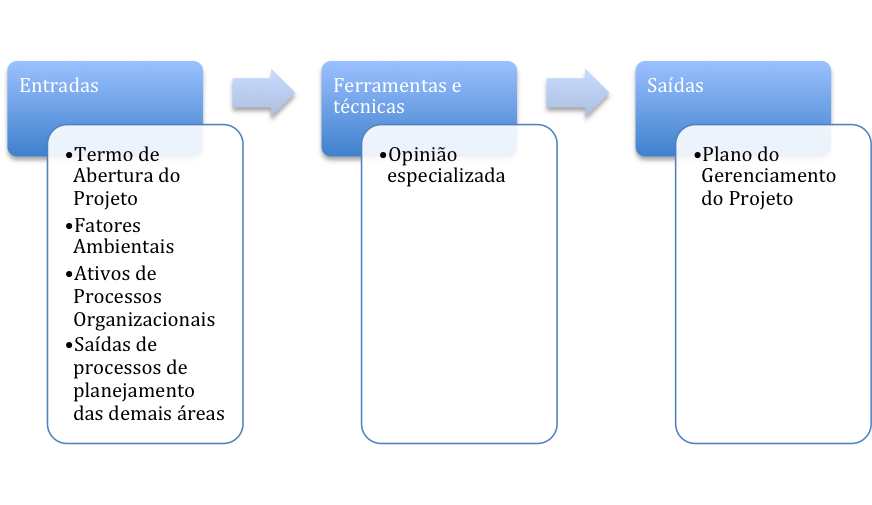
\includegraphics[scale=0.75]{Figuras/proc_integracao_1.png}
\caption{Processo Desenevolver o \planproj}
\label{fig:proc:des:planproj}
\end{figure}

\subsubsection{Entradas}

\begin{itemize}

\item \termo: principal base para início do planejamento, pois possui tudo que ja foi definido para o projeto até o momento.

\item \amb: cultura, infraestrutura, mercado, normas, etc.

\item \ativ: processos e métodos pré-definidos, informações históricas, lições aprendidas, etc.

\item Saidas de processos de planejamento das demais áreas: geram documentos e informações que devem ser integradas para a criação do \planproj. Alterações nestes planos geram alterações no \planproj.

\end{itemize}

\subsubsection{Ferramentas e técnicas}

Opinião especializada:

\begin{itemize}

\item Entender as necessidades do projeto e customizar os processos de acordo

\item Desenvolver e incluir no \planproj detalhes de nível técnico ou gerencial

\item Determinar recursos e conhecimentos necessários para execução do \planproj.

\item Identificar quais documentos necessitam de um processo formal de controle de mudanças.

\end{itemize}

\subsubsection{Saídas}

\planproj.

\subsection{Conteúdo do \planproj}

Além dos demais planos de gerenciamento, o \planproj deve definir:

\begin{itemize}

\item Controle de criação de documentos: quais documentos são necessários, quem tem a responsabilidade de criá-los e quando.

\item Planos auxiliares para gerenciamento das áreas de conhecimento.

\item Linhas de base do escopo, tempo e custo e a formalização dos processos de mudança dessas linhas de base.

\item Processo de controle de mudança:

	\begin{itemize}

	\item Pessoas autorizadas a requisitar mudanças.

	\item Processo de solicitação de mudanças.

	\item Fluxo/processo da mudança:

		\begin{itemize}

		\item Recepção
		\item Análise/avaliação
		\item Classificação
		\item Aprovação
		\item Priorização

		\end{itemize}

\end{itemize}

\end{itemize}
